\documentclass{article}
\usepackage[en]{ukon-infie}
\usepackage[utf8]{inputenc}
\usepackage{algorithm2e}
\usepackage{amsmath}
\usepackage{graphicx}
% kann de oder en sein
% kann bubble break, topexercise sein

\Names{Jonas Probst, Simon Giebenhain, Gabriel Scheibler, Clemens Gutknecht}
\Lecture[DLCV]{Deep Learning for Computer Vision}
\Term{WS 2017/18}

\begin{document}
    \begin{ukon-infie}[24.12.17]{3}

		
		\begin{exercise}[p=20]{Derivatives}
			Let $f: \mathbb{R}^N \rightarrow\mathbb{R}^M$ ,$g: \mathbb{R}^M \times \mathbb{R}^M \rightarrow \mathbb{R}$ and $h:\mathbb{R}^N \rightarrow \mathbb{R}, h(x) := g(f(x), f(x))$. \\
			
			Let $a: \mathbb{R}^N \rightarrow \mathbb{R}^{2M}, a(x) \mapsto (f(x), f(x))$. \\Then $h(x) = g(f(x), f(x)) = g (a(x)) = (g \circ a)(x)$.\\
			Then the following holds for the derivative of $h$.\\
			
			$h'(x) = (g(f(x), f(x)))' = (g(a(x)))' = (g \circ a)'(x)= g'(a(x))a'(x)= g'(f(x), f(x)) (f'(x), f'(x))$. Lets check the dimensions, in order to see if this makes sense:\\
			
			We know that $h'(x) \in \mathbb{R}^{1\times N}$, $g'(f(x), f(x)) \in \mathbb{R}^{1 \times 2M}$ (because $\mathbb{R}^M \times \mathbb{R}^M = \mathbb{R}^{2M}$) and $f'(x) \in \mathbb{R}^{M \times N}$ and therfor $a'(x) = (f'(x),f'(x)) \in \mathbb{R}^{2M \times N}$. Therefor the dimensions of the above equation fit, since $h'(x) \in \mathbb{R}^{1\times N} \text{ and } g'(f(x), f(x)) (f'(x), f'(x)) \in \mathbb{R}^{1\times N}$.
		\end{exercise}
		
		\begin{exercise}[p=25]{Backpropagation}
		\question{}
		{
			Let $g_l: \mathbb{R} \rightarrow \mathbb{R}, y \mapsto (d_l - y)^2$. \\
			With this function we can express the loss in the following way:\\
			$E(w) = \frac{1}{L} \sum_{l=1}^L (g_l \circ f) (x_l, w)$.\\
			With the chain-rule we get the following:\\
			$\frac{\partial E(w)}{\partial w_{1,1}^{2,0}} = \frac{1}{L} \sum_{l=1}^L \frac{\partial}{\partial w_{1,1}^{2,0}}(g_l \circ f) (x_l, w) = \frac{1}{L} \sum_{l=1}^L \frac{\partial g_l(f(x_l,w))}{\partial f(x_l,w)} \frac{\partial}{\partial w_{1,1}^{2,0}}f(x_l, w)  = \frac{1}{L} \sum_{l=1}^L -2(d_l - f(x_l, w))\sum_{j=0}^2 w_{0,j}^{1,1}x_{l_j}$
		}
		
		\question{}
		{ Let $g$ be defined as in a).\\
		
		$\frac{\partial E(w)}{\partial w_{0,1}^{1,0}} = \frac{1}{L} \sum_{l=1}^L \frac{\partial}{\partial w_{0,1}^{1,0}}(g_l \circ f) (x_l, w) = \frac{1}{L} \sum_{l=1}^L \frac{\partial g_l(f(x_l,w))}{\partial f(x_l,w)} \frac{\partial}{\partial w_{0,1}^{1,0}}f(x_l, w)  = \frac{1}{L} \sum_{l=1}^L -2(d_l - f(x_l, w))w_{1,0}^{2,0}x_{l_1}$
		}
		\end{exercise}
		
		\begin{exercise}[p=40+20]{Activation Functions and Batch Normalization}
		\question{}
		{
			We used $\text{leakyReLU}(x) = \text{ReLU}(x) + \alpha \cdot \text{ReLU}(x)$.
		}
		\question{}
		{
			We trained the network with $\alpha$ values ranging from 0 to 1 in 0.1-steps, and obtained the following accuracies:\\
			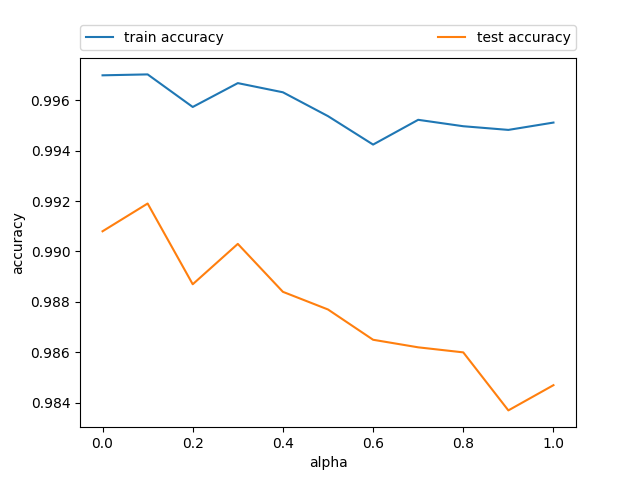
\includegraphics[scale=0.6]{leaky_ReLU_different_alphas.png}\\
			
			One can observe a clear decrease in accuracy, when $\alpha$ gets bigger, however it's unclear what is exactly the best for $\alpha$ in the range of 0 to 0.2.\\
			The source code is in \textbf{leakyRELU.py}
		}
		
		\question{}
		{
			When making $\alpha$ a trainable variable, we obtained the following results:\\
			With 10.000 cycles we got: $\alpha = 0.118417$ with a train accuracy = 0.992 and test accuracy = 0.9902:\\
			With 20.000 cycles we got: $\alpha = 0.093628$ with a train accuracy =  0.9916 and test accuracy =  0.9917:\\
			
			We conclude that the optimal value of $\alpha$ lies around (probably slightly below) 0.1. This coincides with the results b), where 0.1 was the best result.\\
			The source code can be found in \textbf{train\_alpha.py}

		}
		\question{}
		{
			The graph below shows the validation accuracy with and without batch normalization.\\
			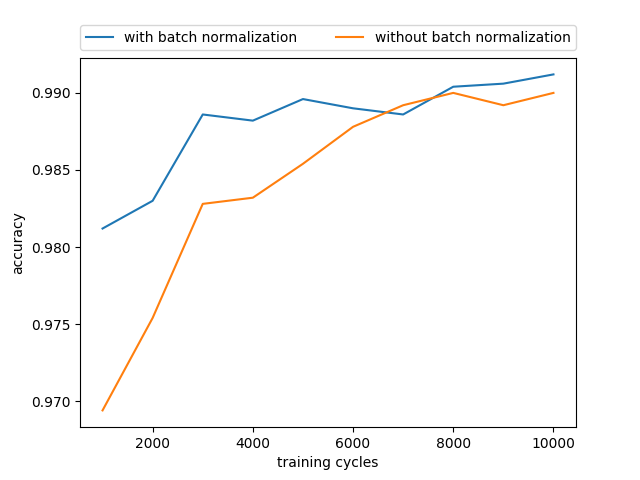
\includegraphics[scale=0.6]{with_vs_without_bn.png}\\
			From the graph above, we observe, that the convergence is much faster with batch normalization. Within the first 1000 training cycles this can be seen most clearly. Regarding the training and testing accuracy, there is not that much difference after a large number of iterations, as can be seen in the following table (small differences don't say much with only 10.000 cycles and only one execution of the expirement):\\
		\begin{tabular}{|l|l|l|}
\hline
               & with bn & without bn \\ \hline
train accuracy & 0.9912  & 0.99       \\ \hline
test accuracy  & 0.9887  & 0.9893     \\ \hline
\end{tabular}\\

The source code can be found in \textbf{batch\_norm.py}

		}
		
		\question{}
		{
			We constructed a deep convolutional net containing 21 residual layers. 7 of these residual layers have 32 features, 7 have 48 and 7 have 64 features. \\
			A residual layer is constructed in the following way:\\
			There are two convolutional layers inside. Each convolutional layer consists of a 3x3 convolution, followed by batch normalization and a ReLU.\\
			At the transition point, where the number of features before and after a residual block inreases, the idendity cannot be added to the result of the convolutions. To make this up, an additional 1x1 convolutional layer is introduced, which constructs the missing features by linearly combining existing ones.\\
			Furthermore we use weight decay. Droput is used in the fully connected layer.\\
			In total we had 42 3x3 conv-layers, 2 1x1 conv-layers and 2 fully connected layers(or 1 I don't know how to count these exactly).\\
			
			The best test accuracy we achieved was 0.994799989462 (after 19.000 training cycles). After 3000 cycles we had 0.993 test accuracy and after 5000 cycles we had 0.9935 test accuracy. This means the the training was relatively fast, and the performance was significantly better than the vanilla version (from the tutorial), which only achieved slightly below 0.992.\\
			The following sums up the training process.\\
			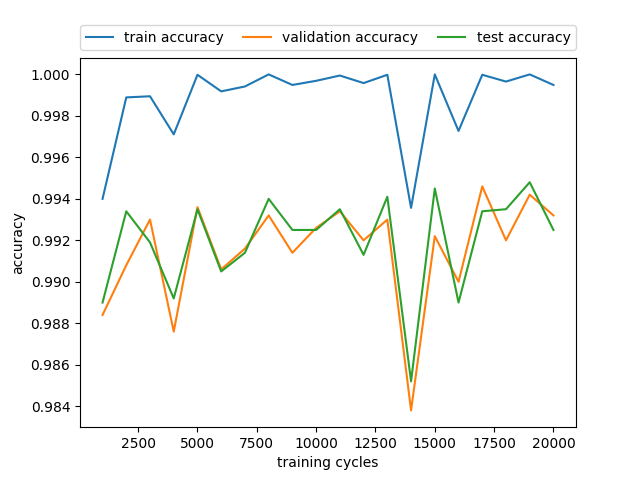
\includegraphics[scale=0.7]{42_layers.png}\\
			The source code can be found in \textbf{deep\_mnist.py}
		}
		\end{exercise}

\end{ukon-infie}
\end{document}
